\begin{figure}
  \begin{tabular}{cc}
    % top row
    %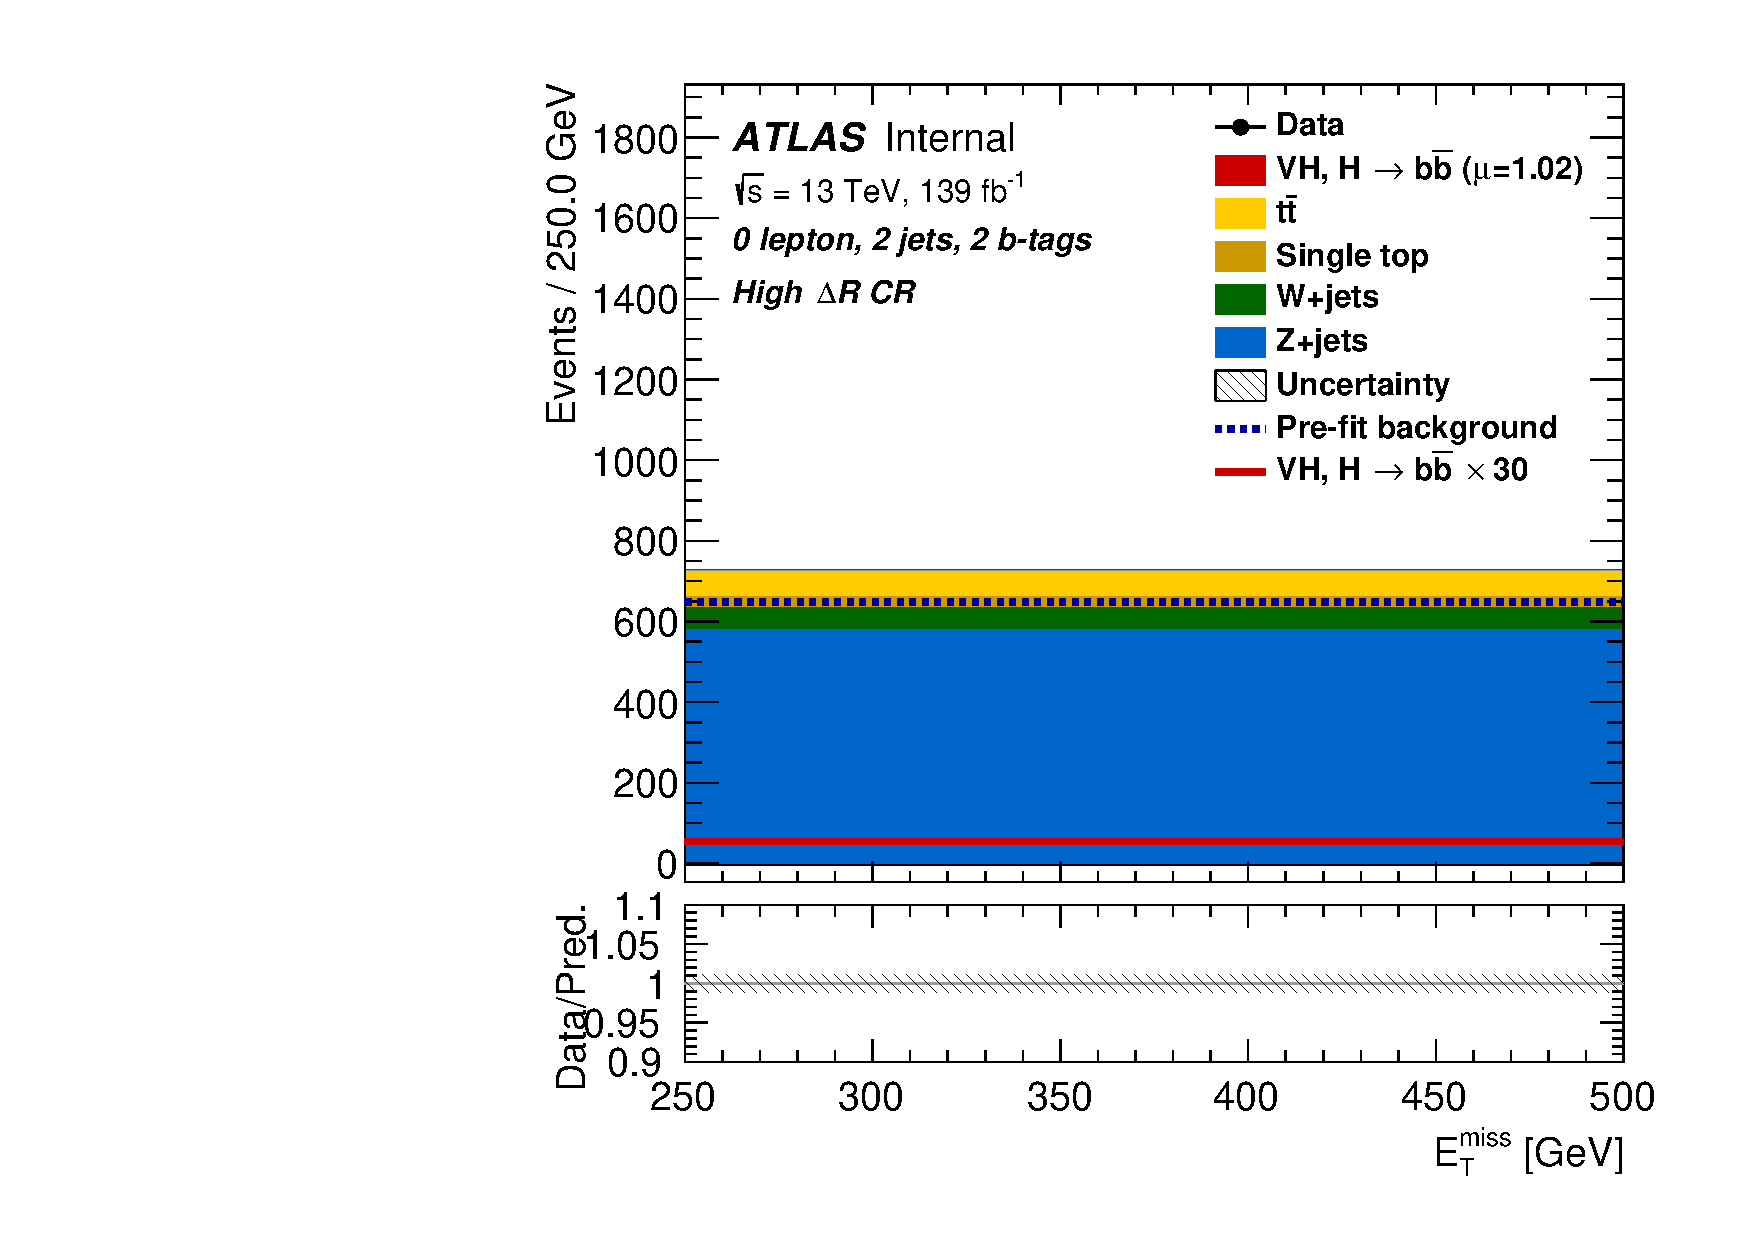
\includegraphics[width=.3\textwidth]{Region_BMin0_Y6051_DCRHigh_T2_L0_distMET_J2_GlobalFit_unconditionnal_mu1}%
    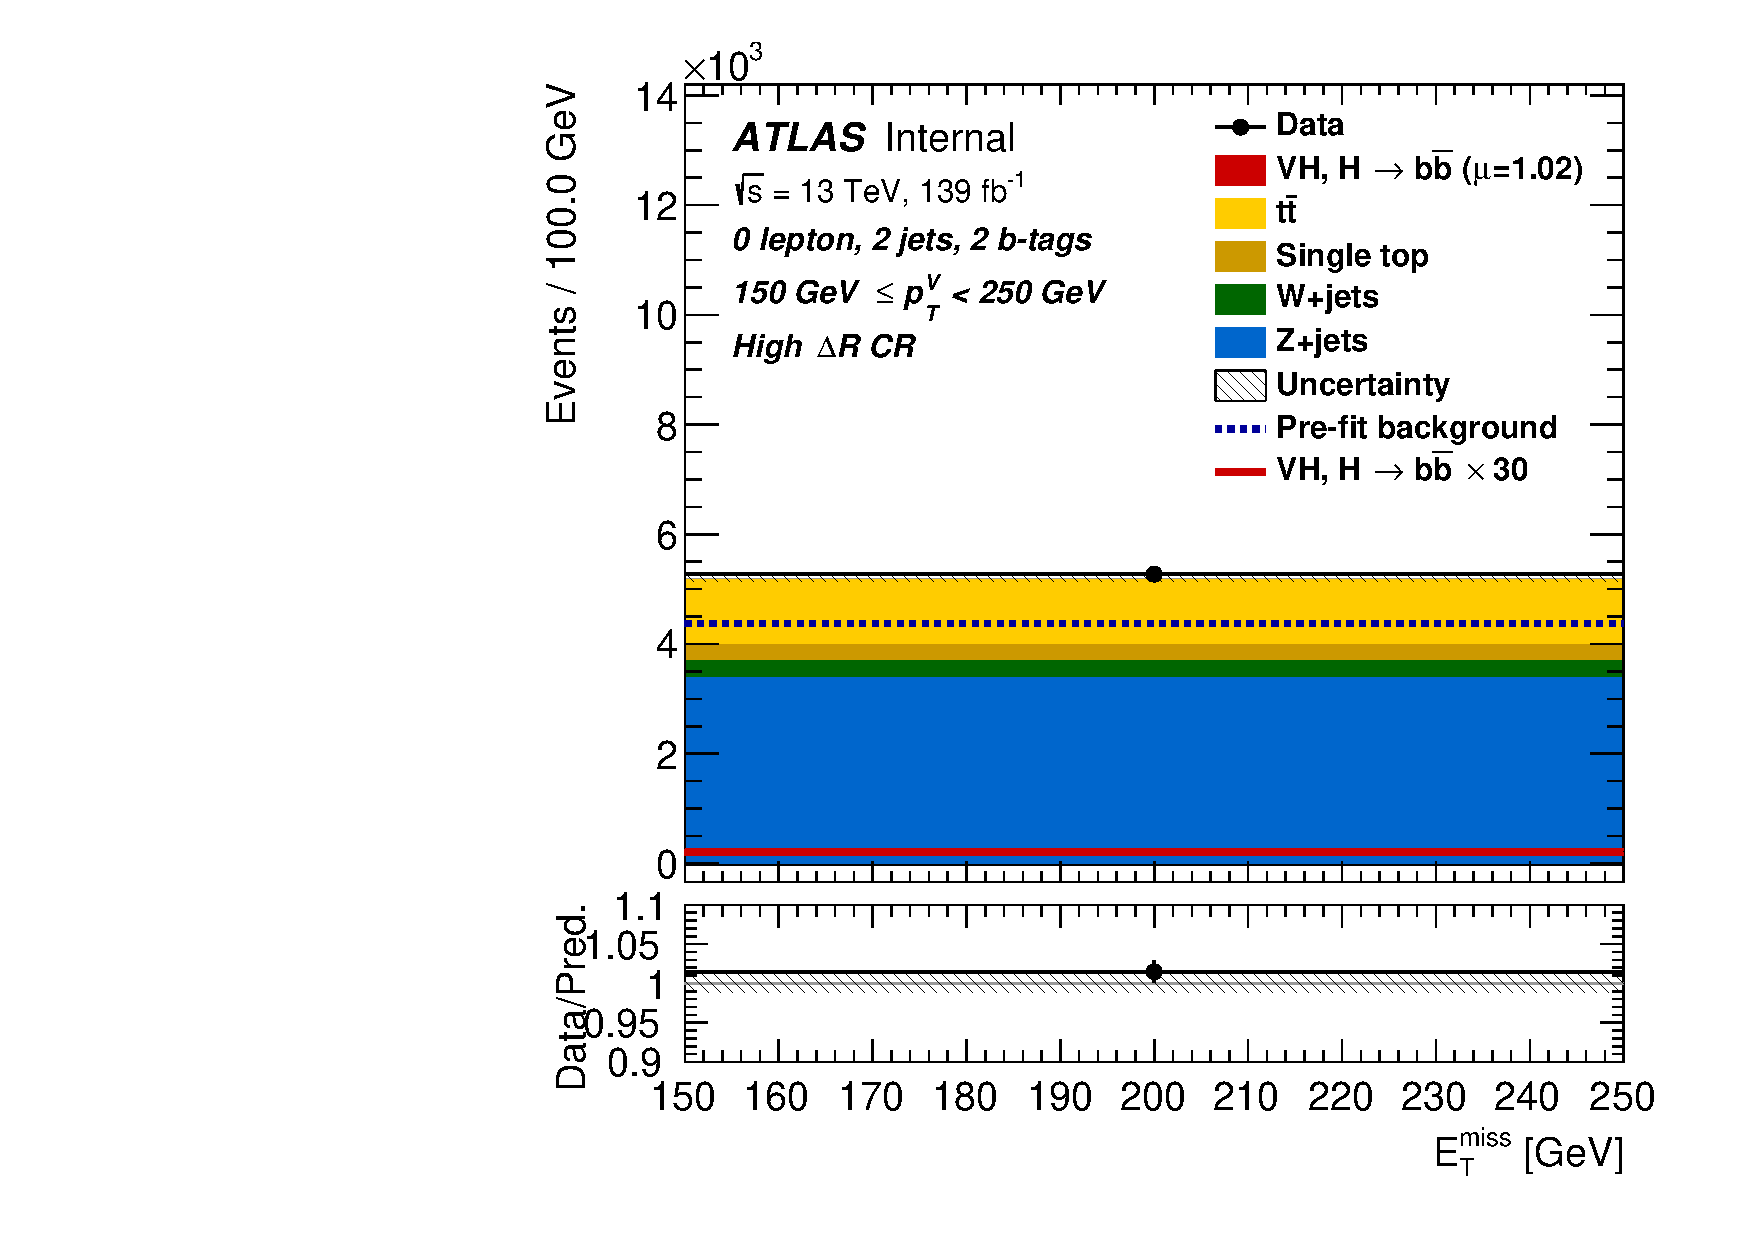
\includegraphics[width=.3\textwidth]{Region_BMax250_BMin150_Y6051_DCRHigh_T2_L0_distMET_J2_GlobalFit_unconditionnal_mu1}%
    & 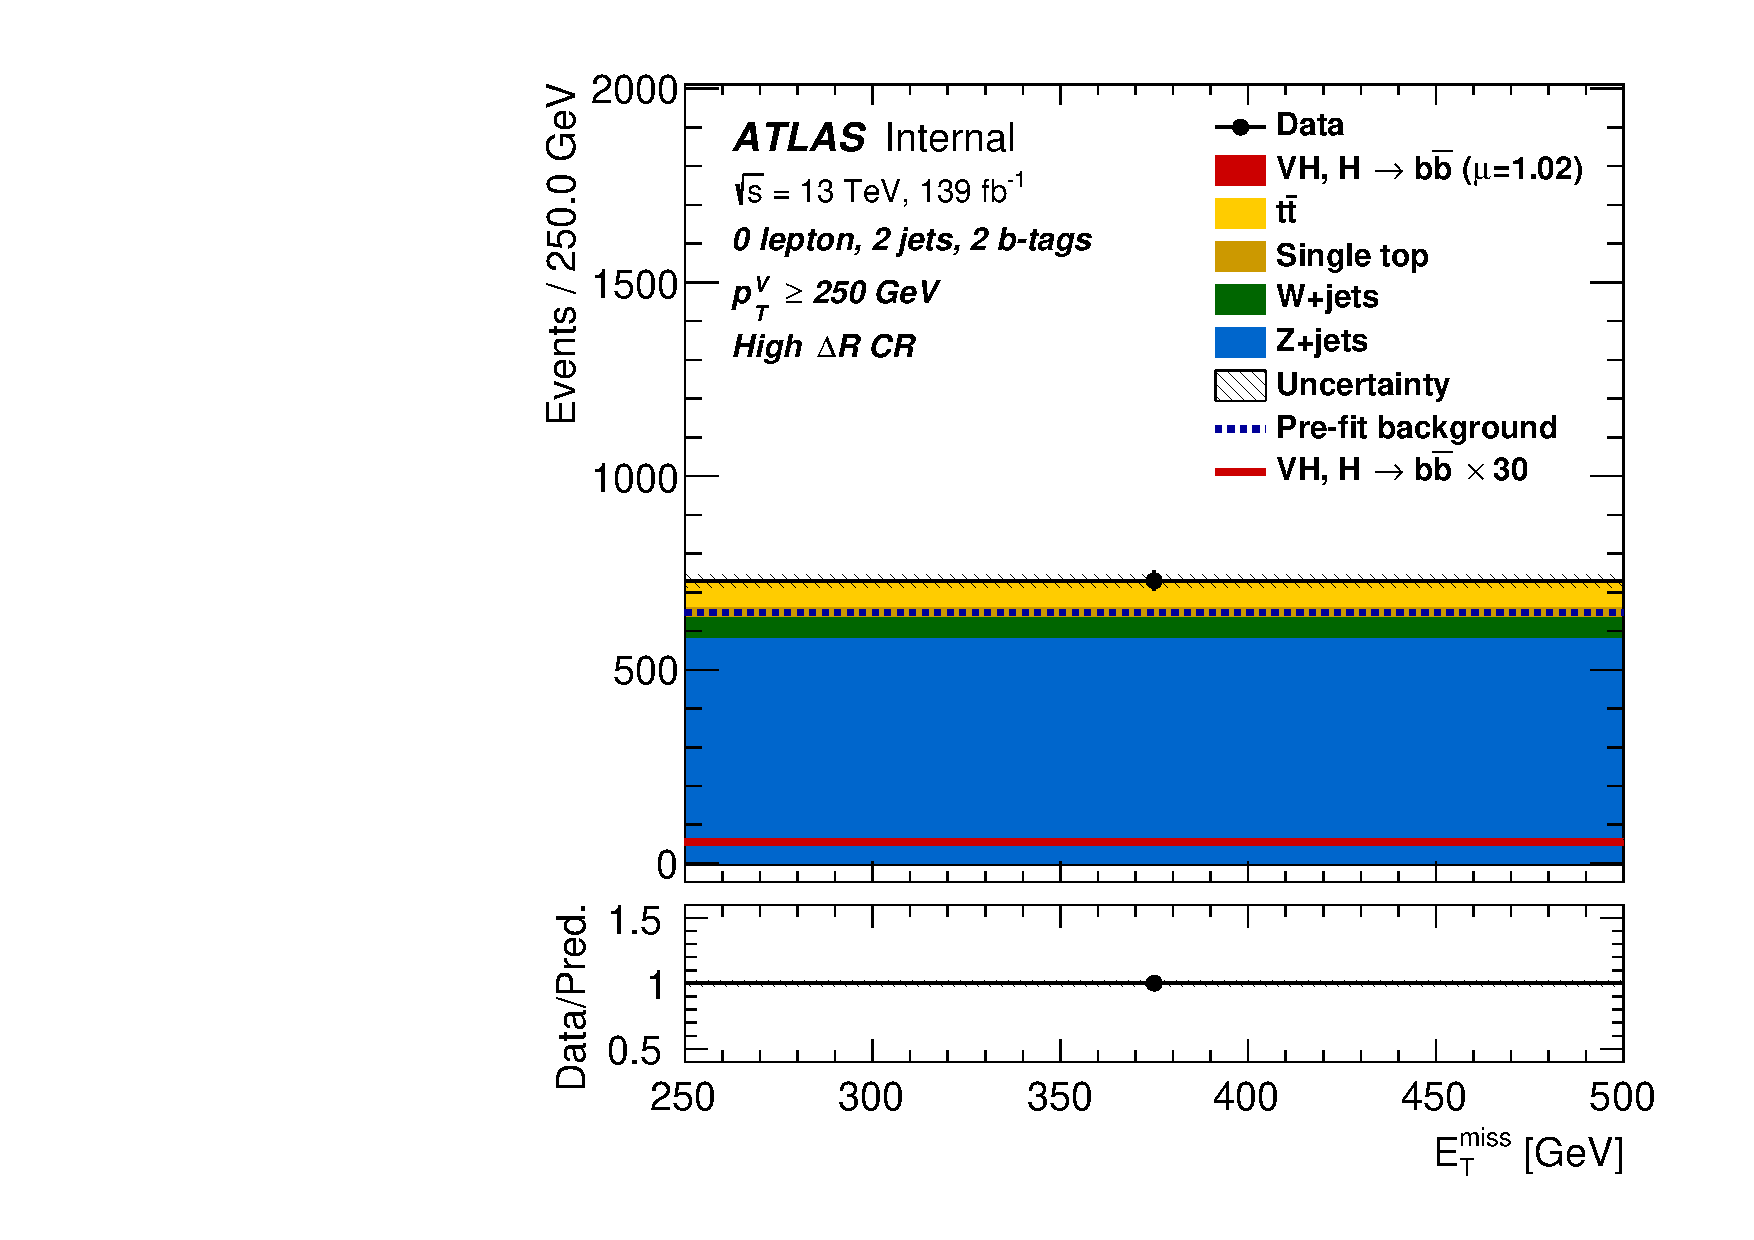
\includegraphics[width=.3\textwidth]{Region_BMin250_Y6051_DCRHigh_T2_L0_distMET_J2_GlobalFit_unconditionnal_mu1} \\

    % middle row
    %\includegraphics[width=.3\textwidth]{}%
    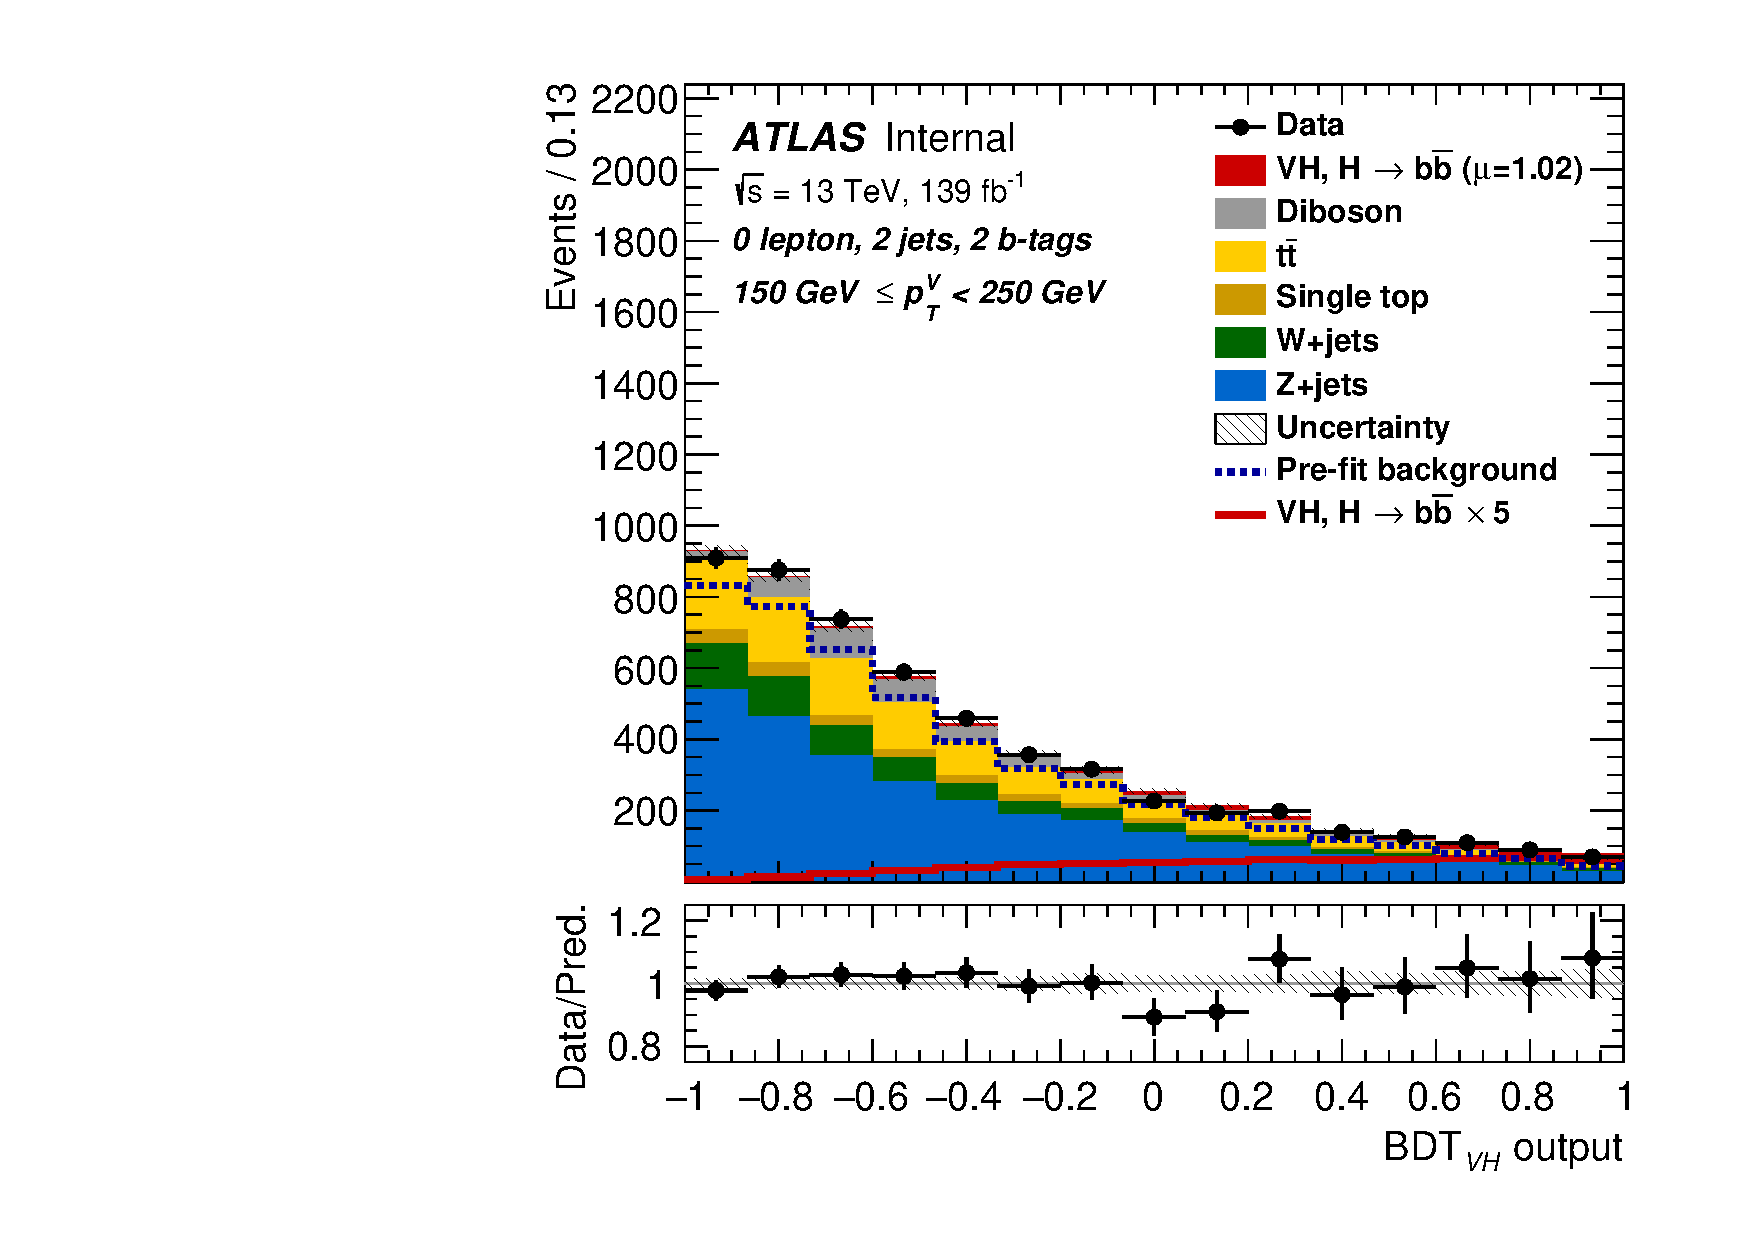
\includegraphics[width=.3\textwidth]{Region_BMax250_BMin150_Y6051_DSR_T2_L0_distmva_J2_GlobalFit_unconditionnal_mu1}%
    & 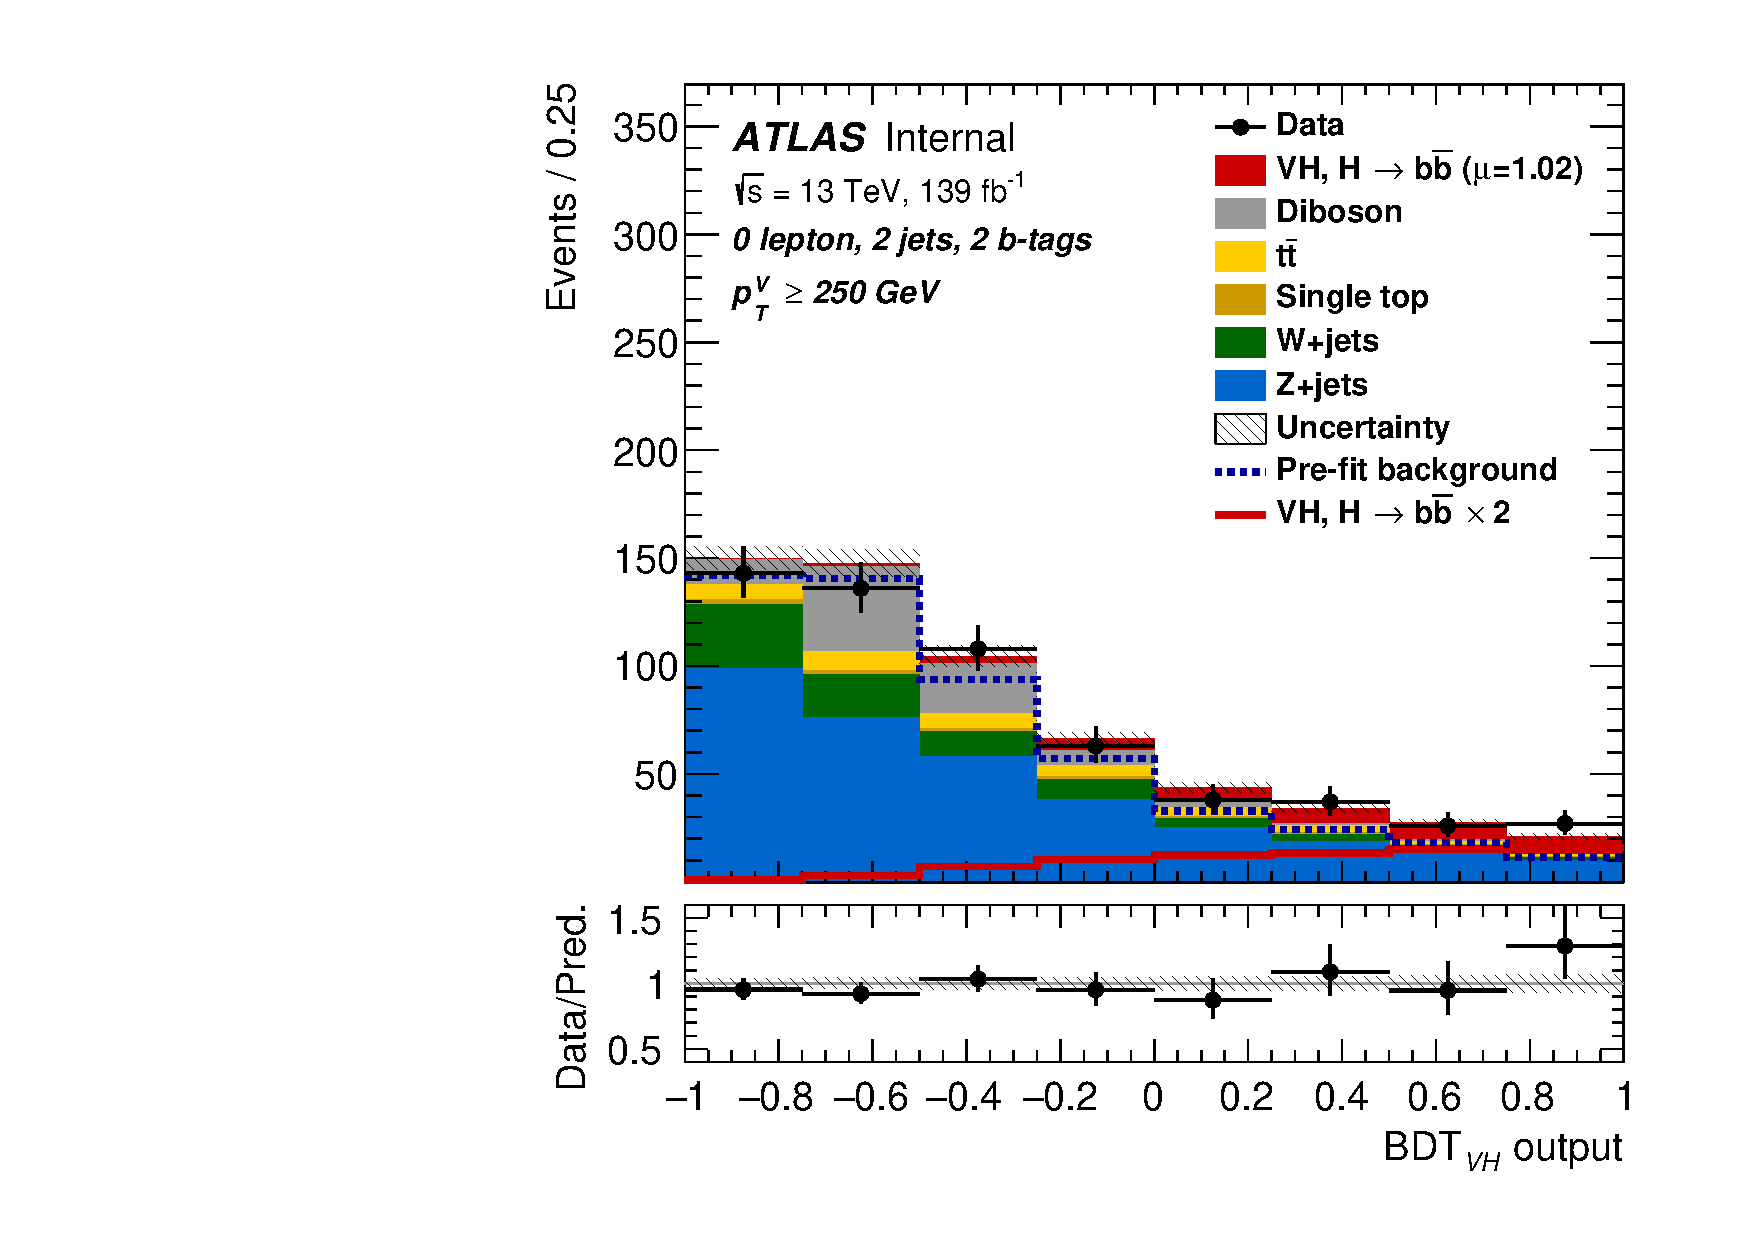
\includegraphics[width=.3\textwidth]{Region_BMin250_Y6051_DSR_T2_L0_distmva_J2_GlobalFit_unconditionnal_mu1} \\

    % bottom row
    %\includegraphics[width=.3\textwidth]{it}%
    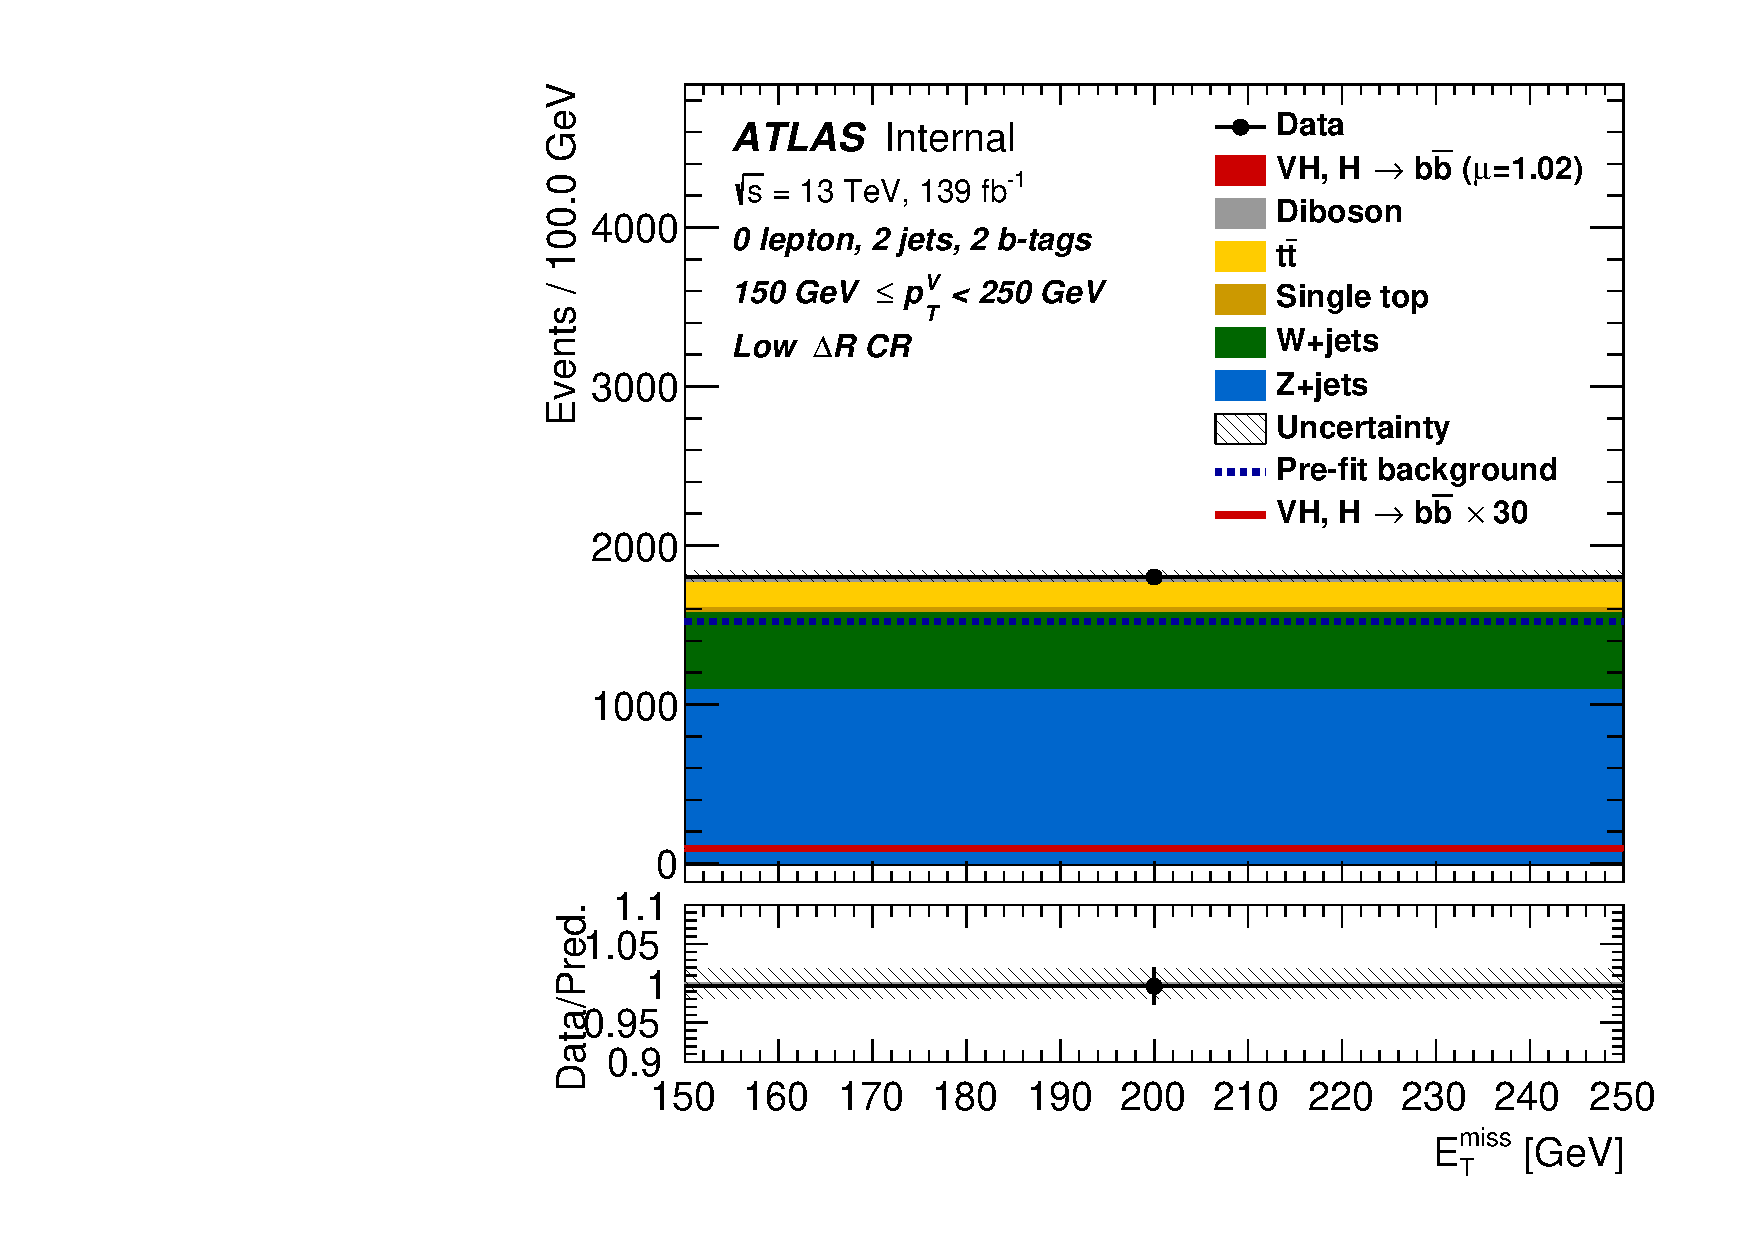
\includegraphics[width=.3\textwidth]{Region_BMax250_BMin150_Y6051_DCRLow_T2_L0_distMET_J2_GlobalFit_unconditionnal_mu1}%
    & 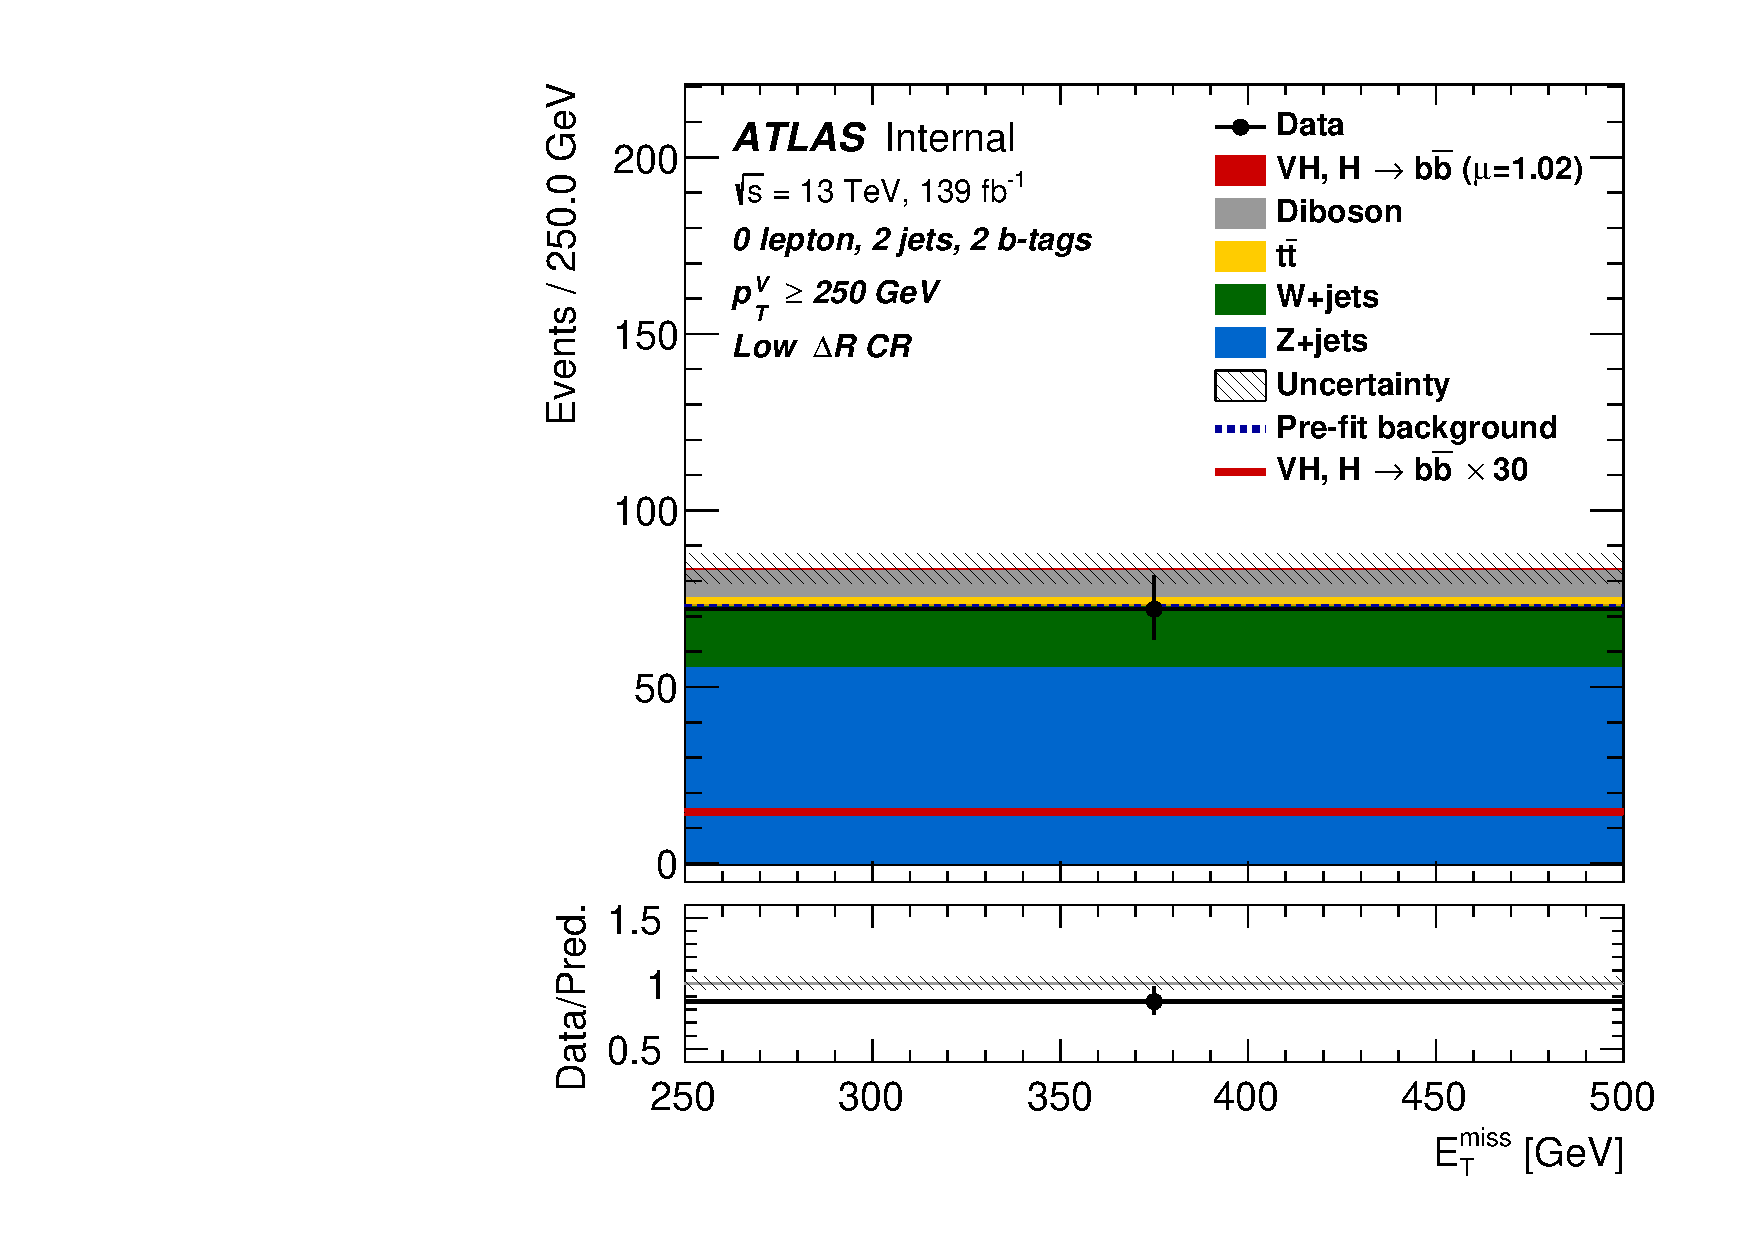
\includegraphics[width=.3\textwidth]{Region_BMin250_Y6051_DCRLow_T2_L0_distMET_J2_GlobalFit_unconditionnal_mu1} \\
    
    % (a) first & (b) second \\[6pt]
    %(c) third & (d) fourth \\[6pt]
    %\multicolumn{2}{c}{\includegraphics[width=65mm]{it} }\\
    %\multicolumn{2}{c}{(e) fifth}
  \end{tabular}
  \caption{caption}
\end{figure}